\documentclass[]{article}
\usepackage{lmodern}
\usepackage{amssymb,amsmath}
\usepackage{ifxetex,ifluatex}
\usepackage{fixltx2e} % provides \textsubscript
\ifnum 0\ifxetex 1\fi\ifluatex 1\fi=0 % if pdftex
  \usepackage[T1]{fontenc}
  \usepackage[utf8]{inputenc}
\else % if luatex or xelatex
  \ifxetex
    \usepackage{mathspec}
  \else
    \usepackage{fontspec}
  \fi
  \defaultfontfeatures{Ligatures=TeX,Scale=MatchLowercase}
\fi
% use upquote if available, for straight quotes in verbatim environments
\IfFileExists{upquote.sty}{\usepackage{upquote}}{}
% use microtype if available
\IfFileExists{microtype.sty}{%
\usepackage{microtype}
\UseMicrotypeSet[protrusion]{basicmath} % disable protrusion for tt fonts
}{}
\usepackage[margin=1in]{geometry}
\usepackage{hyperref}
\hypersetup{unicode=true,
            pdftitle={Introducing the funneljoin package},
            pdfauthor={Emily Robinson},
            pdfborder={0 0 0},
            breaklinks=true}
\urlstyle{same}  % don't use monospace font for urls
\usepackage{color}
\usepackage{fancyvrb}
\newcommand{\VerbBar}{|}
\newcommand{\VERB}{\Verb[commandchars=\\\{\}]}
\DefineVerbatimEnvironment{Highlighting}{Verbatim}{commandchars=\\\{\}}
% Add ',fontsize=\small' for more characters per line
\usepackage{framed}
\definecolor{shadecolor}{RGB}{248,248,248}
\newenvironment{Shaded}{\begin{snugshade}}{\end{snugshade}}
\newcommand{\KeywordTok}[1]{\textcolor[rgb]{0.13,0.29,0.53}{\textbf{#1}}}
\newcommand{\DataTypeTok}[1]{\textcolor[rgb]{0.13,0.29,0.53}{#1}}
\newcommand{\DecValTok}[1]{\textcolor[rgb]{0.00,0.00,0.81}{#1}}
\newcommand{\BaseNTok}[1]{\textcolor[rgb]{0.00,0.00,0.81}{#1}}
\newcommand{\FloatTok}[1]{\textcolor[rgb]{0.00,0.00,0.81}{#1}}
\newcommand{\ConstantTok}[1]{\textcolor[rgb]{0.00,0.00,0.00}{#1}}
\newcommand{\CharTok}[1]{\textcolor[rgb]{0.31,0.60,0.02}{#1}}
\newcommand{\SpecialCharTok}[1]{\textcolor[rgb]{0.00,0.00,0.00}{#1}}
\newcommand{\StringTok}[1]{\textcolor[rgb]{0.31,0.60,0.02}{#1}}
\newcommand{\VerbatimStringTok}[1]{\textcolor[rgb]{0.31,0.60,0.02}{#1}}
\newcommand{\SpecialStringTok}[1]{\textcolor[rgb]{0.31,0.60,0.02}{#1}}
\newcommand{\ImportTok}[1]{#1}
\newcommand{\CommentTok}[1]{\textcolor[rgb]{0.56,0.35,0.01}{\textit{#1}}}
\newcommand{\DocumentationTok}[1]{\textcolor[rgb]{0.56,0.35,0.01}{\textbf{\textit{#1}}}}
\newcommand{\AnnotationTok}[1]{\textcolor[rgb]{0.56,0.35,0.01}{\textbf{\textit{#1}}}}
\newcommand{\CommentVarTok}[1]{\textcolor[rgb]{0.56,0.35,0.01}{\textbf{\textit{#1}}}}
\newcommand{\OtherTok}[1]{\textcolor[rgb]{0.56,0.35,0.01}{#1}}
\newcommand{\FunctionTok}[1]{\textcolor[rgb]{0.00,0.00,0.00}{#1}}
\newcommand{\VariableTok}[1]{\textcolor[rgb]{0.00,0.00,0.00}{#1}}
\newcommand{\ControlFlowTok}[1]{\textcolor[rgb]{0.13,0.29,0.53}{\textbf{#1}}}
\newcommand{\OperatorTok}[1]{\textcolor[rgb]{0.81,0.36,0.00}{\textbf{#1}}}
\newcommand{\BuiltInTok}[1]{#1}
\newcommand{\ExtensionTok}[1]{#1}
\newcommand{\PreprocessorTok}[1]{\textcolor[rgb]{0.56,0.35,0.01}{\textit{#1}}}
\newcommand{\AttributeTok}[1]{\textcolor[rgb]{0.77,0.63,0.00}{#1}}
\newcommand{\RegionMarkerTok}[1]{#1}
\newcommand{\InformationTok}[1]{\textcolor[rgb]{0.56,0.35,0.01}{\textbf{\textit{#1}}}}
\newcommand{\WarningTok}[1]{\textcolor[rgb]{0.56,0.35,0.01}{\textbf{\textit{#1}}}}
\newcommand{\AlertTok}[1]{\textcolor[rgb]{0.94,0.16,0.16}{#1}}
\newcommand{\ErrorTok}[1]{\textcolor[rgb]{0.64,0.00,0.00}{\textbf{#1}}}
\newcommand{\NormalTok}[1]{#1}
\usepackage{graphicx,grffile}
\makeatletter
\def\maxwidth{\ifdim\Gin@nat@width>\linewidth\linewidth\else\Gin@nat@width\fi}
\def\maxheight{\ifdim\Gin@nat@height>\textheight\textheight\else\Gin@nat@height\fi}
\makeatother
% Scale images if necessary, so that they will not overflow the page
% margins by default, and it is still possible to overwrite the defaults
% using explicit options in \includegraphics[width, height, ...]{}
\setkeys{Gin}{width=\maxwidth,height=\maxheight,keepaspectratio}
\IfFileExists{parskip.sty}{%
\usepackage{parskip}
}{% else
\setlength{\parindent}{0pt}
\setlength{\parskip}{6pt plus 2pt minus 1pt}
}
\setlength{\emergencystretch}{3em}  % prevent overfull lines
\providecommand{\tightlist}{%
  \setlength{\itemsep}{0pt}\setlength{\parskip}{0pt}}
\setcounter{secnumdepth}{0}
% Redefines (sub)paragraphs to behave more like sections
\ifx\paragraph\undefined\else
\let\oldparagraph\paragraph
\renewcommand{\paragraph}[1]{\oldparagraph{#1}\mbox{}}
\fi
\ifx\subparagraph\undefined\else
\let\oldsubparagraph\subparagraph
\renewcommand{\subparagraph}[1]{\oldsubparagraph{#1}\mbox{}}
\fi

%%% Use protect on footnotes to avoid problems with footnotes in titles
\let\rmarkdownfootnote\footnote%
\def\footnote{\protect\rmarkdownfootnote}

%%% Change title format to be more compact
\usepackage{titling}

% Create subtitle command for use in maketitle
\providecommand{\subtitle}[1]{
  \posttitle{
    \begin{center}\large#1\end{center}
    }
}

\setlength{\droptitle}{-2em}

  \title{Introducing the funneljoin package}
    \pretitle{\vspace{\droptitle}\centering\huge}
  \posttitle{\par}
    \author{Emily Robinson}
    \preauthor{\centering\large\emph}
  \postauthor{\par}
      \predate{\centering\large\emph}
  \postdate{\par}
    \date{2019-07-26}


\begin{document}
\maketitle

Have you ever had a ``first this then that'' question? For example,
maybe you're an e-commerce business and you want all the times people
clicked on an item and then added it to their cart within 2 days, or the
last page they visited before registering. Or
\href{https://twitter.com/scottishnp/status/1154657704578695168?s=20}{you
work with pharmaceutical data} and need to know what drugs people took
before drug x and which drugs they took afterward and when. Or you
\href{https://twitter.com/Voovarb/status/1154445792125394945?s=20}{tag
fish} and need to know where they went and if they eventually migrated
upstream.

Enter the funneljoin package. The goal of funneljoin is to make it easy
to analyze behavior funnels with the \texttt{after\_join()},
\texttt{funnel\_start()}, and \texttt{funnel\_step()} functions. If you
work with data where you have events with their time and associated
user, you probably have a problem funneljoin can help with. I created
this package with \href{https://twitter.com/drob}{David Robinson} and
\href{https://www.linkedin.com/in/awbaker1/}{Anthony Baker} in July 2018
and have continued to maintain and build on it since.

In this post, I'll use \texttt{funneljoin::after\_join()} to analyze
data about all Stack Overflow questions and answers (including their
other tags) with the tag R up to September 24th, 2017. The data was
downloaded from Kaggle
\href{https://www.kaggle.com/stackoverflow/rquestions/downloads/rquestions.zip/3}{here}.
The next post in this series will look at the \texttt{funnel\_start()}
and \texttt{funnel\_step()} functions, which we'll use when all of the
events or behavior are in one table.

\subsection{Set-up}\label{set-up}

\begin{Shaded}
\begin{Highlighting}[]
\KeywordTok{library}\NormalTok{(knitr)}
\NormalTok{opts_chunk}\OperatorTok{$}\KeywordTok{set}\NormalTok{(}\DataTypeTok{message =} \OtherTok{FALSE}\NormalTok{, }\DataTypeTok{warning =} \OtherTok{FALSE}\NormalTok{, }\DataTypeTok{fig.width =} \DecValTok{12} \OperatorTok{*}\StringTok{ }\NormalTok{.}\DecValTok{8}\NormalTok{, }\DataTypeTok{fig.height =} \DecValTok{8} \OperatorTok{*}\StringTok{ }\NormalTok{.}\DecValTok{8}\NormalTok{)}
\end{Highlighting}
\end{Shaded}

\begin{Shaded}
\begin{Highlighting}[]
\KeywordTok{library}\NormalTok{(tidyverse)}

\NormalTok{answers <-}\StringTok{ }\KeywordTok{read_csv}\NormalTok{(}\StringTok{"Answers.csv"}\NormalTok{)}
\NormalTok{questions <-}\StringTok{ }\KeywordTok{read_csv}\NormalTok{(}\StringTok{"Questions.csv"}\NormalTok{)}
\end{Highlighting}
\end{Shaded}

\texttt{funneljoin} is not yet on CRAN, so you'll need to use
\texttt{devtools} to install it from GitHub. I'll also use Ciarán
Tobin's package \texttt{ggthemr} to set my ggplot2 theme; check out the
palettes available on the
\href{https://github.com/cttobin/ggthemr}{GitHub page}.

\begin{Shaded}
\begin{Highlighting}[]
\CommentTok{# devtools::install_github("robinsones/funneljoin")}
\KeywordTok{library}\NormalTok{(funneljoin)}
\end{Highlighting}
\end{Shaded}

\begin{Shaded}
\begin{Highlighting}[]
\CommentTok{# devtools::install_github('cttobin/ggthemr')}
\KeywordTok{library}\NormalTok{(ggthemr)}
\KeywordTok{ggthemr}\NormalTok{(}\StringTok{'fresh'}\NormalTok{)}
\end{Highlighting}
\end{Shaded}

Let's take a quick look at the questions and answers data set.

\begin{Shaded}
\begin{Highlighting}[]
\NormalTok{questions}
\end{Highlighting}
\end{Shaded}

\begin{verbatim}
## # A tibble: 189,930 x 6
##        Id OwnerUserId CreationDate        Score Title         Body         
##     <dbl>       <dbl> <dttm>              <dbl> <chr>         <chr>        
##  1  77434       14008 2008-09-16 21:40:29   171 How to acces~ "<p>Suppose ~
##  2  79709          NA 2008-09-17 03:39:16     3 Worse sin: s~ "<p>I have a~
##  3  95007       15842 2008-09-18 17:59:19    56 Explain the ~ "<p>I've bee~
##  4 103312          NA 2008-09-19 16:09:26     4 How to test ~ "<p>How can ~
##  5 255697     1941213 2008-11-01 15:48:30     4 Is there an ~ "<p>I'm look~
##  6 359438        2173 2008-12-11 14:02:06     4 Optimization~ "<p>Does any~
##  7 439526       37751 2009-01-13 15:58:48    23 Thinking in ~ "<p>I know t~
##  8 445059       37751 2009-01-14 23:09:02    12 Vectorize my~ "<p>So earli~
##  9 467110       11301 2009-01-21 21:33:13     5 Is R a compi~ "<p>I can't ~
## 10 476726         277 2009-01-24 21:56:23    10 Filtering da~ "<p>I have a~
## # ... with 189,920 more rows
\end{verbatim}

\begin{Shaded}
\begin{Highlighting}[]
\NormalTok{answers }
\end{Highlighting}
\end{Shaded}

\begin{verbatim}
## # A tibble: 250,788 x 7
##       Id OwnerUserId CreationDate        ParentId Score IsAcceptedAnswer
##    <dbl>       <dbl> <dttm>                 <dbl> <dbl> <lgl>           
##  1 79741        3259 2008-09-17 03:43:22    79709    -1 FALSE           
##  2 79768        6043 2008-09-17 03:48:29    79709     9 FALSE           
##  3 79779        8002 2008-09-17 03:49:36    79709     0 FALSE           
##  4 79788          NA 2008-09-17 03:51:30    79709     4 FALSE           
##  5 79827       14257 2008-09-17 03:58:26    79709     1 FALSE           
##  6 79893       14928 2008-09-17 04:11:08    79709     6 FALSE           
##  7 83162       15842 2008-09-17 13:27:17    77434    70 FALSE           
##  8 83222        1428 2008-09-17 13:32:45    77434   236 FALSE           
##  9 86804          NA 2008-09-17 19:39:37    79709     1 FALSE           
## 10 95598        1179 2008-09-18 18:49:09    95007     5 FALSE           
## # ... with 250,778 more rows, and 1 more variable: Body <chr>
\end{verbatim}

Before I dive into the analysis, I'm going to use the janitor's package
\texttt{clean\_names()} function to convert the column names to snake
case and \texttt{\%\textless{}\textgreater{}\%} to modify the data sets.
I'll also get rid of the rows where user id is missing.

\begin{Shaded}
\begin{Highlighting}[]
\KeywordTok{library}\NormalTok{(magrittr)}

\NormalTok{questions }\OperatorTok
\StringTok{  }\NormalTok{janitor}\OperatorTok{::}\KeywordTok{clean_names}\NormalTok{() }\OperatorTok
\StringTok{  }\KeywordTok{filter}\NormalTok{(}\OperatorTok{!}\KeywordTok{is.na}\NormalTok{(owner_user_id))}

\NormalTok{answers }\OperatorTok
\StringTok{  }\NormalTok{janitor}\OperatorTok{::}\KeywordTok{clean_names}\NormalTok{() }\OperatorTok
\StringTok{  }\KeywordTok{filter}\NormalTok{(}\OperatorTok{!}\KeywordTok{is.na}\NormalTok{(owner_user_id))}
\end{Highlighting}
\end{Shaded}

\subsection{after\_join()}\label{after_join}

Let's start with a relatively simple question - how many people who ask
a question later answer one? To look at this, we'll need to link the
questions with the answers table using \texttt{owner\_user\_id} and
\texttt{creation\_date} using funneljoin's \texttt{after\_join}
function.

\begin{Shaded}
\begin{Highlighting}[]
\KeywordTok{after_join}\NormalTok{(questions, }
\NormalTok{           answers,}
           \DataTypeTok{by_time =} \StringTok{"creation_date"}\NormalTok{,}
           \DataTypeTok{by_user =} \StringTok{"owner_user_id"}\NormalTok{,}
           \DataTypeTok{mode =} \StringTok{"left"}\NormalTok{,}
           \DataTypeTok{type =} \StringTok{"first-firstafter"}\NormalTok{)}
\end{Highlighting}
\end{Shaded}

\begin{verbatim}
## # A tibble: 60,335 x 12
##      id.x owner_user_id creation_date.x     score.x title body.x    id.y
##     <dbl>         <dbl> <dttm>                <dbl> <chr> <chr>    <dbl>
##  1  77434         14008 2008-09-16 21:40:29     171 How ~ "<p>S~      NA
##  2  95007         15842 2008-09-18 17:59:19      56 Expl~ "<p>I~ 4249121
##  3 255697       1941213 2008-11-01 15:48:30       4 Is t~ "<p>I~      NA
##  4 359438          2173 2008-12-11 14:02:06       4 Opti~ "<p>D~      NA
##  5 439526         37751 2009-01-13 15:58:48      23 Thin~ "<p>I~  440066
##  6 467110         11301 2009-01-21 21:33:13       5 Is R~ "<p>I~      NA
##  7 476726           277 2009-01-24 21:56:23      10 Filt~ "<p>I~ 4727309
##  8 495744         12677 2009-01-30 14:48:19       2 Oper~ "<p>I~ 2203628
##  9 498932           445 2009-01-31 14:50:28       3 What~ "<p>I~  511763
## 10 520810         63372 2009-02-06 15:49:48      20 Does~ "<p>A~      NA
## # ... with 60,325 more rows, and 5 more variables: creation_date.y <dttm>,
## #   parent_id <dbl>, score.y <dbl>, is_accepted_answer <lgl>, body.y <chr>
\end{verbatim}

The first two arguments are the tables we're joining, with the first
table being the events that happen first. We then specify what the time
and user id columns are and the mode of the join (e.g.~left, inner,
anti).

The power of \texttt{after\_join()} comes in its \texttt{type} argument,
which allows you to switch between types of funnels easily. In this
case, we wanted only the first question someone asked and then wanted to
know the first answer they gave afterward. For any \texttt{type} of
\texttt{after\_join()} though, the time stamps of the second table (in
this case answers) will always be after the time stamp of the first
table for each user - we can see their are no rows where
\texttt{creation\_date.y} (the time of the answer) is before
\texttt{creation\_date.x} (the time of the question):

\begin{Shaded}
\begin{Highlighting}[]
\KeywordTok{after_join}\NormalTok{(questions, }
\NormalTok{           answers,}
           \DataTypeTok{by_time =} \StringTok{"creation_date"}\NormalTok{,}
           \DataTypeTok{by_user =} \StringTok{"owner_user_id"}\NormalTok{,}
           \DataTypeTok{mode =} \StringTok{"left"}\NormalTok{,}
           \DataTypeTok{type =} \StringTok{"first-firstafter"}\NormalTok{) }\OperatorTok
\StringTok{  }\KeywordTok{filter}\NormalTok{(creation_date.y }\OperatorTok{<}\StringTok{ }\NormalTok{creation_date.x)}
\end{Highlighting}
\end{Shaded}

\begin{verbatim}
## # A tibble: 0 x 12
## # ... with 12 variables: id.x <dbl>, owner_user_id <dbl>,
## #   creation_date.x <dttm>, score.x <dbl>, title <chr>, body.x <chr>,
## #   id.y <dbl>, creation_date.y <dttm>, parent_id <dbl>, score.y <dbl>,
## #   is_accepted_answer <lgl>, body.y <chr>
\end{verbatim}

Because we wanted to keep all users even if they never answered a
question later, we do a left join, specified with
\texttt{mode\ =\ "left"}.

To answer our original question, let's get a count by what percent of
rows don't have an \texttt{id.y}, meaning they never answered a question
after asking one. We'll use the funneljoin's
\texttt{summarize\_conversions()} function, where you specify what
column indicates whether someone ``converted'' (in this case answered a
question) and returns the total number of users (\texttt{nb\_users}),
the number of conversions (\texttt{nb\_conversions}), and the percent
converted (\texttt{pct\_converted}).

\begin{Shaded}
\begin{Highlighting}[]
\KeywordTok{after_join}\NormalTok{(questions, }
\NormalTok{                answers,}
                \DataTypeTok{by_time =} \StringTok{"creation_date"}\NormalTok{,}
                \DataTypeTok{by_user =} \StringTok{"owner_user_id"}\NormalTok{,}
                \DataTypeTok{type =} \StringTok{"first-firstafter"}\NormalTok{,}
                \DataTypeTok{mode =} \StringTok{"left"}\NormalTok{) }\OperatorTok
\StringTok{  }\KeywordTok{summarize_conversions}\NormalTok{(}\DataTypeTok{converted =}\NormalTok{ id.y)}
\end{Highlighting}
\end{Shaded}

\begin{verbatim}
## # A tibble: 1 x 3
##   nb_users nb_conversions pct_converted
##      <int>          <int>         <dbl>
## 1    60335          13688         0.227
\end{verbatim}

We see that of the approximately 60,000 users that asked an R question,
22.7\% percent later went on to answer one.

How long does it take for people to answer their first question? We can
add \texttt{gap\_col\ =\ TRUE} to \texttt{after\_join()} to add a
column, \texttt{.gap}, which is the gap between events (in seconds).
We'll also switch from from using the argument \texttt{mode} to specify
the type of join to changing to a wrapper function,
\texttt{after\_left\_join()}.

\begin{Shaded}
\begin{Highlighting}[]
\NormalTok{questions }\OperatorTok
\StringTok{  }\KeywordTok{after_left_join}\NormalTok{(answers,}
                  \DataTypeTok{by_time =} \StringTok{"creation_date"}\NormalTok{,}
                  \DataTypeTok{by_user =} \StringTok{"owner_user_id"}\NormalTok{,}
                  \DataTypeTok{type =} \StringTok{"first-firstafter"}\NormalTok{,}
                  \DataTypeTok{gap_col =} \OtherTok{TRUE}\NormalTok{) }\OperatorTok
\StringTok{  }\KeywordTok{mutate}\NormalTok{(}\DataTypeTok{gap_hours =}\NormalTok{ .gap  }\OperatorTok{/}\StringTok{ }\DecValTok{3600}\NormalTok{) }\OperatorTok
\StringTok{  }\KeywordTok{ggplot}\NormalTok{(}\KeywordTok{aes}\NormalTok{(}\DataTypeTok{x =}\NormalTok{ gap_hours)) }\OperatorTok{+}\StringTok{ }
\StringTok{  }\KeywordTok{geom_histogram}\NormalTok{() }\OperatorTok{+}\StringTok{ }
\StringTok{  }\KeywordTok{scale_x_log10}\NormalTok{(}\DataTypeTok{breaks =} \KeywordTok{c}\NormalTok{(}\DecValTok{1}\NormalTok{, }\DecValTok{24}\NormalTok{, }\DecValTok{24} \OperatorTok{*}\StringTok{ }\DecValTok{7}\NormalTok{, }\DecValTok{24} \OperatorTok{*}\StringTok{ }\DecValTok{7} \OperatorTok{*}\StringTok{ }\DecValTok{30}\NormalTok{), }
                     \DataTypeTok{labels =} \KeywordTok{c}\NormalTok{(}\StringTok{"1 hour"}\NormalTok{, }\StringTok{"1 day"}\NormalTok{, }\StringTok{"1 week"}\NormalTok{, }\StringTok{"1 month"}\NormalTok{)) }\OperatorTok{+}\StringTok{ }
\StringTok{  }\KeywordTok{labs}\NormalTok{(}\DataTypeTok{x =} \StringTok{""}\NormalTok{,}
       \DataTypeTok{y =} \StringTok{"Number of users"}\NormalTok{,}
       \DataTypeTok{title =} \StringTok{"What's the gap between someone's first StackOverflow question and their first answer?"}\NormalTok{,}
       \DataTypeTok{subtitle =} \StringTok{"Only for questions tagged with R"}\NormalTok{) }
\end{Highlighting}
\end{Shaded}

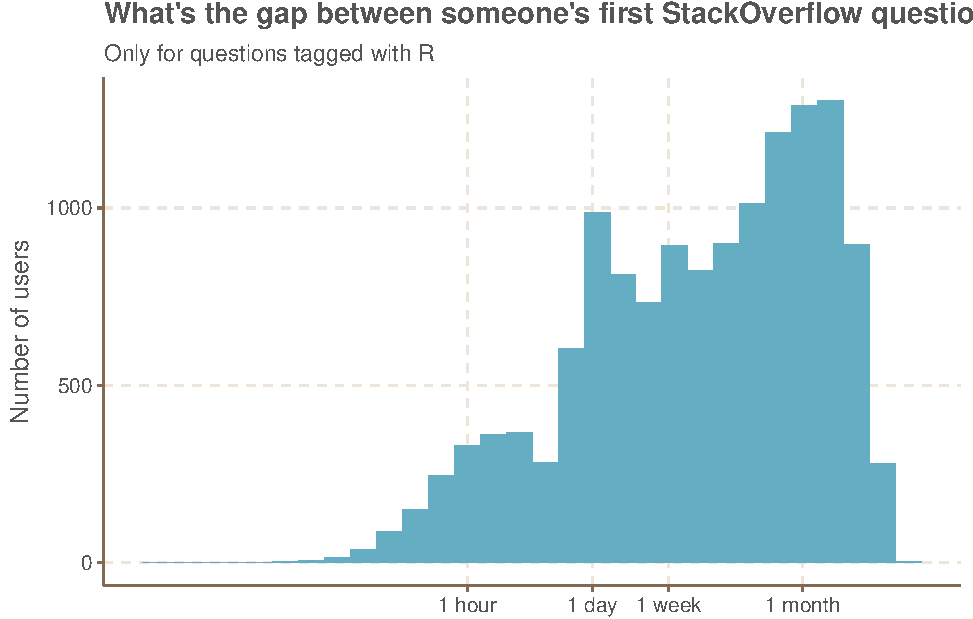
\includegraphics{2019-07-25-introducing-the-funneljoin-package_files/figure-latex/unnamed-chunk-11-1.pdf}

We can get an idea from this graph what percentage of people who ask a
question answer one within a week, or we could filter our data to get an
exact answer. To make it even easier though, we can use the
\texttt{max\_gap} argument in \texttt{after\_join()} to specify that
someone needs to have answered a question within a week from their data
to be joined. \texttt{max\_gap} takes either a \texttt{difftime} or an
integer representing the gap in seconds and will filter so that the time
between events is less than or equal to that \texttt{max\_gap}.

\begin{Shaded}
\begin{Highlighting}[]
\KeywordTok{after_join}\NormalTok{(questions, }
\NormalTok{           answers,}
           \DataTypeTok{by_time =} \StringTok{"creation_date"}\NormalTok{,}
           \DataTypeTok{by_user =} \StringTok{"owner_user_id"}\NormalTok{,}
           \DataTypeTok{type =} \StringTok{"first-firstafter"}\NormalTok{,}
           \DataTypeTok{mode =} \StringTok{"left"}\NormalTok{,}
           \DataTypeTok{max_gap =} \KeywordTok{as.difftime}\NormalTok{(}\DecValTok{1}\NormalTok{, }\DataTypeTok{units =} \StringTok{"weeks"}\NormalTok{)) }\OperatorTok
\StringTok{  }\KeywordTok{summarize_conversions}\NormalTok{(}\DataTypeTok{converted =}\NormalTok{ id.y)}
\end{Highlighting}
\end{Shaded}

\begin{verbatim}
## # A tibble: 1 x 3
##   nb_users nb_conversions pct_converted
##      <int>          <int>         <dbl>
## 1    60335           5349        0.0887
\end{verbatim}

Now we see that only 8.9\% answer an R question within a week of asking
their first one.

We might be curious if the likelihood of answering a question later
varies by the score of the question they asked. Before doing
summarize\_conversions, we can group by the score. There are some scores
that only appear once (e.g.~one person got a score of -18), so we'll
filter for only scores where there were more than 100 questions that got
that score.

\begin{Shaded}
\begin{Highlighting}[]
\KeywordTok{after_join}\NormalTok{(questions, }
\NormalTok{           answers,}
           \DataTypeTok{by_time =} \StringTok{"creation_date"}\NormalTok{,}
           \DataTypeTok{by_user =} \StringTok{"owner_user_id"}\NormalTok{,}
           \DataTypeTok{type =} \StringTok{"first-firstafter"}\NormalTok{,}
           \DataTypeTok{mode =} \StringTok{"left"}\NormalTok{) }\OperatorTok
\StringTok{  }\KeywordTok{group_by}\NormalTok{(score.x) }\OperatorTok
\StringTok{  }\KeywordTok{summarize_conversions}\NormalTok{(}\DataTypeTok{converted =}\NormalTok{ id.y) }\OperatorTok
\StringTok{  }\KeywordTok{filter}\NormalTok{(nb_users }\OperatorTok{>}\StringTok{ }\DecValTok{100}\NormalTok{) }\OperatorTok
\StringTok{  }\KeywordTok{ggplot}\NormalTok{(}\KeywordTok{aes}\NormalTok{(}\DataTypeTok{x =}\NormalTok{ score.x, }\DataTypeTok{y =}\NormalTok{ pct_converted)) }\OperatorTok{+}\StringTok{ }
\StringTok{  }\KeywordTok{geom_line}\NormalTok{() }\OperatorTok{+}\StringTok{ }
\StringTok{  }\KeywordTok{geom_point}\NormalTok{(}\KeywordTok{aes}\NormalTok{(}\DataTypeTok{size =}\NormalTok{ nb_users)) }\OperatorTok{+}\StringTok{ }
\StringTok{  }\KeywordTok{scale_y_continuous}\NormalTok{(}\DataTypeTok{labels =}\NormalTok{ scales}\OperatorTok{::}\NormalTok{percent) }\OperatorTok{+}\StringTok{ }
\StringTok{  }\KeywordTok{labs}\NormalTok{(}\DataTypeTok{y =} \StringTok{"% who later answer a question"}\NormalTok{,}
      \DataTypeTok{x =} \StringTok{"Score on a user's first question"}\NormalTok{,}
      \DataTypeTok{title =} \StringTok{"If your first question is scored highly, you're more to answer a question later"}\NormalTok{,}
      \DataTypeTok{subtitle =} \StringTok{"Only for questions tagged with R"}\NormalTok{,}
      \DataTypeTok{size =} \StringTok{"Number of users"}\NormalTok{) }\OperatorTok{+}\StringTok{ }
\StringTok{  }\KeywordTok{expand_limits}\NormalTok{(}\DataTypeTok{y =} \DecValTok{0}\NormalTok{)}
\end{Highlighting}
\end{Shaded}

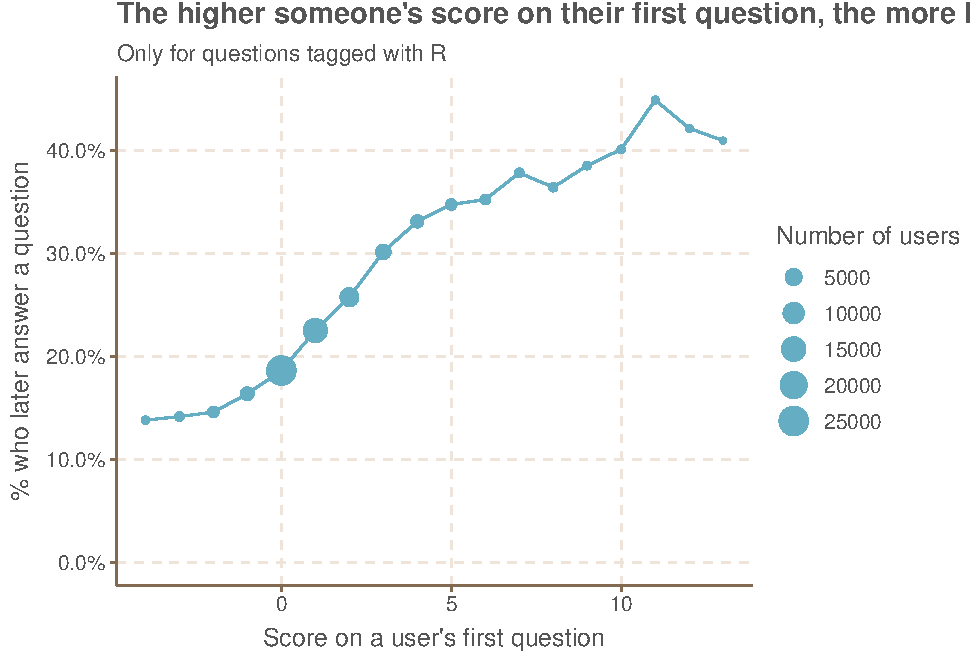
\includegraphics{2019-07-25-introducing-the-funneljoin-package_files/figure-latex/unnamed-chunk-13-1.pdf}

Most people's first questions have a score between -1 and 4, but for
those who manage to score higher, they're more likely to answer a
question later. As always, you have to be careful of any claims of
causality: it's likely be those who are asking higher scored questions
are better at R and thus have the knowledge to later provide answers.

We've been looking so far at people's answers after they've asked a
question. But are there people who answer a question before they ever
ask one? We can examine this with a \texttt{after\_right\_join} (to keep
everyone who asks a question) to see what percent have answered one
before. A \texttt{first-first} filters each table to the first instance
of a user (e.g.~their first answer and their first question) and then
will only keep answers if it happened before the question.

\begin{Shaded}
\begin{Highlighting}[]
\NormalTok{answers }\OperatorTok
\StringTok{  }\KeywordTok{after_join}\NormalTok{(questions,}
           \DataTypeTok{by_time =} \StringTok{"creation_date"}\NormalTok{,}
           \DataTypeTok{by_user =} \StringTok{"owner_user_id"}\NormalTok{,}
           \DataTypeTok{type =} \StringTok{"first-first"}\NormalTok{,}
           \DataTypeTok{mode =} \StringTok{"right"}\NormalTok{) }\OperatorTok
\StringTok{  }\KeywordTok{summarize_conversions}\NormalTok{(id.x)}
\end{Highlighting}
\end{Shaded}

\begin{verbatim}
## # A tibble: 1 x 3
##   nb_users nb_conversions pct_converted
##      <int>          <int>         <dbl>
## 1    60335           2795        0.0463
\end{verbatim}

Yes, 4.63\% of people have answered a question before they asked their
first one.

To answer our original question, we used a \texttt{first-firstafter}
type join, which means we've only been getting one row per user. For
people who answer questions after asking one, let's find out how many
they answer. We'll switch our query to an \texttt{after\_inner\_join}
with a type \texttt{first-any}. Each user will only have one question,
their first, as we used a \texttt{first-Y} type. But it has one row per
answer they gave afterwards as we used a \texttt{X-any} type.

\begin{Shaded}
\begin{Highlighting}[]
\NormalTok{questions }\OperatorTok
\StringTok{  }\KeywordTok{after_inner_join}\NormalTok{(answers,}
           \DataTypeTok{by_time =} \StringTok{"creation_date"}\NormalTok{,}
           \DataTypeTok{by_user =} \StringTok{"owner_user_id"}\NormalTok{,}
           \DataTypeTok{type =} \StringTok{"first-any"}\NormalTok{) }\OperatorTok
\StringTok{  }\KeywordTok{count}\NormalTok{(owner_user_id) }\OperatorTok
\StringTok{  }\KeywordTok{ggplot}\NormalTok{(}\KeywordTok{aes}\NormalTok{(n)) }\OperatorTok{+}\StringTok{ }
\StringTok{  }\KeywordTok{geom_histogram}\NormalTok{() }\OperatorTok{+}\StringTok{ }
\StringTok{  }\KeywordTok{scale_x_log10}\NormalTok{() }\OperatorTok{+}\StringTok{ }
\StringTok{  }\KeywordTok{labs}\NormalTok{(}\DataTypeTok{x =} \StringTok{"Number of answers"}\NormalTok{,}
       \DataTypeTok{y =} \StringTok{"Number of users"}\NormalTok{,}
       \DataTypeTok{title =} \StringTok{"How many questions do people answer after asking their first one?"}\NormalTok{,}
       \DataTypeTok{subtitle =} \StringTok{"Only for questions tagged with R on StackOverflow and people who answer at least one"}\NormalTok{)}
\end{Highlighting}
\end{Shaded}

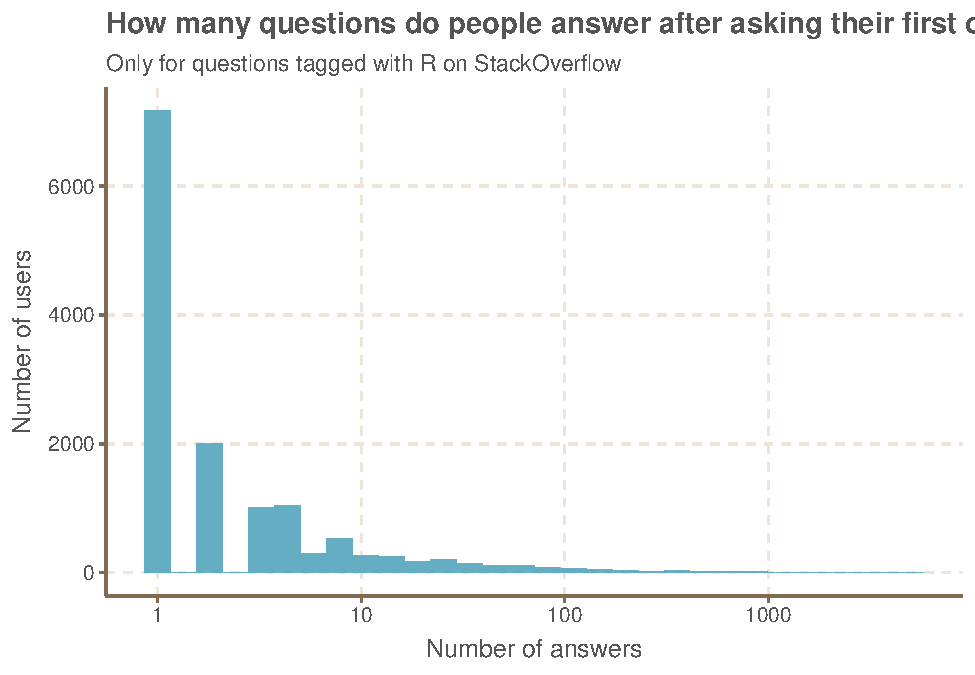
\includegraphics{2019-07-25-introducing-the-funneljoin-package_files/figure-latex/unnamed-chunk-15-1.pdf}

Not surprisingly, we see people mostly answer only 1 or 2 questions,
with a long-tail of power users answering 100+ questions.

\subsection{Conclusion}\label{conclusion}

Some of the power of \texttt{funneljoin} comes from making it possible
to code things you didn't know how to before. But a lot of it comes from
bringing things from ``possible but time-consuming/annoying'' to
``easy.'' When you're doing exploratory analysis, you want to be able to
quickly iterate between ideas: switching from the first thing someone
added to their cart after searching for an item, to everything they
added, to only things they added within a week.

In the next post, I'll be sharing \texttt{funneljoin}'s other main
functions: \texttt{funnel\_start()} and \texttt{funnel\_step()}. In the
meantime, if you find any bugs or have a feature request or question,
please create an issue on
\href{https://github.com/robinsones/funneljoin}{GitHub} or get in touch
on \href{https://twitter.com/robinson_es}{Twitter}!


\end{document}
